\documentclass[a4paper,10pt]{article}
\input{/Users/WannaGetHigh/workspace/latex/macros.tex}

\title{Multi touch support implementation in Pharo}
\author{Fran�ois \bsc{Lepan}\\Benjamin \bsc{Van Ryseghem}}

\begin{document}
\maketitle

\vfill
\section*{Introduction}
During our project our main goal was to introduce a new way to handle multi touch events and gesture in Pharo.
Starting from what we previously did in last semester during the PJE lecture, we used the same approach to
introduce a handling of gestures based on TUIO with an architecture allowing to switch to virtual machine events.

In order to analyse these gestures we needed a state machine that would fill the gap between the human gesture
and a perfect gesture. This state machine got better over the time we added gestures but still isn't perfect.

Another goal was to clean and reunify the whole hierarchy of system events and to provide a clean abstraction
of low level data structure.

\vfill
\vfill
\newpage
\tableofcontents
\newpage

\section{TUOI and blobs analysis}
	
Our first goal is to be able to retrieve gesture from the user. In order to do so we used TUIO which is a protocol for 
multitouch events. It retrieve the multi-touch gesture from the user on a surface and then generate events for each 
finger on the surface (\emph{cf}~Fig.~\ref{fig:TUIO_platform_diagram}). For our tests we used a small software called 
Tongseng that generate TUIO events from the trackpad and a small library created by our tutor that parse the TUIO events.

\section{System events hierarchy}
\section{Switching to VM events}
\section{State machine limits}
\section{Gesture implementation}
\section{Conclusion}

\section{Appendices}

\begin{figure}[ht]
\begin{center}
	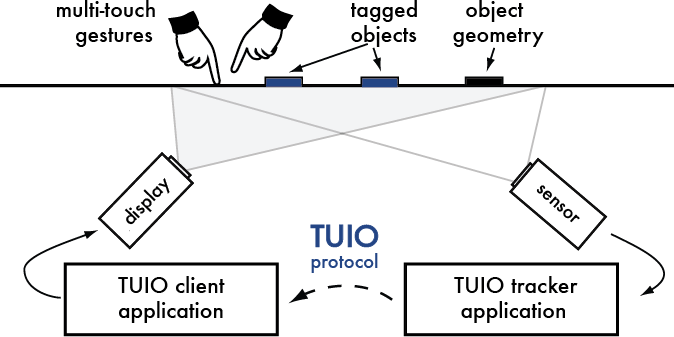
\includegraphics[width=15cm]{figures/TUIO_platform_diagram.png}
\end{center}
	\caption{Diagram of the TUIO protocol}
	\label{fig:TUIO_platform_diagram}
\end{figure}


%\signature

\end{document}